\documentclass[letterpaper,10pt,conference]{ieeeconf}
\IEEEoverridecommandlockouts
\overrideIEEEmargins
\usepackage{fontspec}
\setmainfont{Times New Roman}
\setsansfont{Arial}
\setmonofont{Menlo}
\usepackage{amsmath,amssymb,graphicx,booktabs,cite,url}
\graphicspath{{figures/}}
\newcommand{\R}{\mathbb{R}}
\newcommand{\vct}[1]{\vec{#1}}
\newcommand{\CornerSpeed}{$0.285\,\mathrm{m/s}$}
\newcommand{\NoRollSpeed}{$0.137\,\mathrm{m/s}$}
\newcommand{\PairSpeed}{$0.278\,\mathrm{m/s}$}
\newcommand{\MJVersion}{3.10.0}

\title{\LARGE\bf Task-Space Travel Allocation for an Articulated Arc-Leg Hexapod}
\author{\mbox{}}
\begin{document}
\maketitle
\thispagestyle{empty}\pagestyle{empty}
\begin{abstract}
An actuated arc at the end of an articulated leg can serve as both a support foot and a rolling surface. Exploiting this shared joint is difficult: superposing a rolling command on a full walking trajectory can demand the same contact travel twice, while a finite arc must be repositioned before its opening reaches the ground. We present a geometry-based controller for a six-legged, eighteen-actuator platform. It assigns rolling or stepping roles according to steering feasibility, allocates contact travel between sector rotation and articulation, and reindexes finite sectors within alternating-tripod swing windows. A deterministic MuJoCo study crosses five controller restrictions, two forward commands, and eight initial phases. At a commanded $0.45\,\mathrm{m/s}$, the four-corner configuration achieves \CornerSpeed{} against \NoRollSpeed{} for the same scheduler with rolling disabled; a two-leg configuration achieves \PairSpeed{}. These are net-displacement speeds, not instantaneous peaks. We report tracking error, mechanical work, slip, and phase dependence alongside speed. Collision inspection shows that the current single-mesh tire proxy fills the arc's inner concavity, preventing attribution of stair ascent to inner-edge hooking. The results support a bounded simulation study of travel allocation; quantitative hardware validation of this controller, concave-contact advantages, and general terrain robustness remain open. Archival prototype photographs are presented separately from the new simulations.
\end{abstract}

\section{Introduction}
An incomplete circular contact at a leg tip offers a useful form of actuator reuse. Holding its distal joint can provide a planted support, rotating it can transport the body, and moving the upstream joints can place the contact elsewhere. These possibilities do not automatically produce a coherent hybrid gait. The rolling direction may be poorly aligned with the required contact motion, steering changes the footprint, and the finite sector eventually runs out of supporting material. Increasing distal speed without addressing these constraints can increase slip instead of useful displacement.

The problem is particularly visible in an articulated hexapod. For one body command, some legs may be well oriented to roll while others must step. A controller that assigns every leg the same behavior ignores this geometric asymmetry. Conversely, separate walking and rolling commands can compete if each independently accounts for the full commanded displacement. We therefore formulate locomotion around a single budget: the body-relative travel required at each ground contact. Rolling supplies its feasible component, and articulation supplies the remainder.

The contribution is a concrete realization of this allocation on an eighteen-actuator arc-leg model, including finite-sector handling and a controlled comparison of rolling-leg subsets. The geometric construction uses the distal rotation axis and contact radius, rather than the displacement of the lowest geometric mesh point, to infer rolling direction. Roles and steering are latched at lift-off, and a grounded rolling leg skips a scheduled swing when sufficient usable arc remains. The evaluation isolates the complete role-allocation mechanism against its rolling-disabled restriction on the same model and gait settings. It also compares two-leg and four-leg rolling subsets and a separate tripod scheduler with the same cadence and stride caps.

We make three bounded claims. First, geometric feasibility can select different roles within one commanded motion. Second, allocating a portion of contact travel to bounded sector rotation can increase net forward transport relative to the rolling-disabled scheduler in the tested model. Third, the number and placement of rolling legs changes the speed--tracking--work trade-off. We do not claim the first hybrid leg-wheel robot, optimal role selection, improved battery efficiency, or quantitative hardware validation of the proposed controller.

\begin{figure}[t]
\centering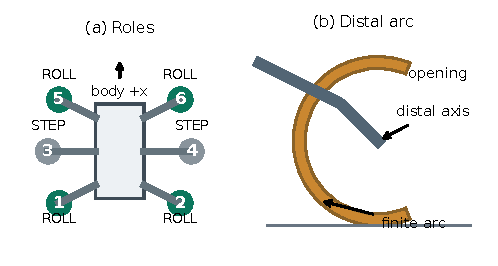
\includegraphics[width=\columnwidth]{concept.pdf}
\caption{Conceptual geometry and control allocation (schematic, not a measured robot pose). A finite distal arc reuses the third leg joint for rotation. Under a forward command the corner legs can qualify for rolling, while the middle pair steps. IDs follow the model; ``forward'' is the initial chassis $x$ direction.}
\label{fig:concept}
\end{figure}

\begin{figure}[t]
\centering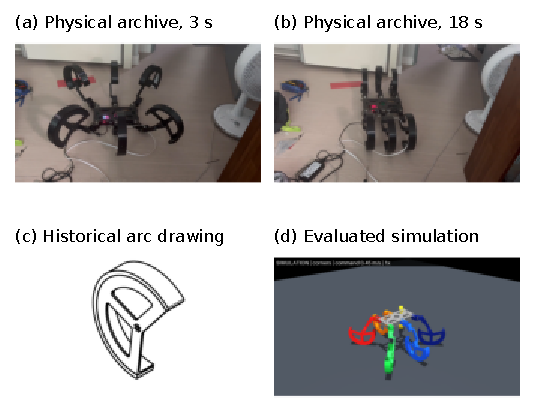
\includegraphics[width=\columnwidth]{platform.pdf}
\caption{Physical prototype and evaluated model. (a,b) Frames at 3 and 18 s of an archival floor-motion clip, showing different limb arrangements and visible external cables. (c) Arc component in the historical fabrication drawing, cropped to remove its title block. (d) Newly rendered model at the nominal pose. The archive establishes embodiment; it is not a hardware trial of the controller evaluated here.}
\label{fig:platform}
\end{figure}

\section{Related Work and Research Question}
Continuously rotating curved legs predate this platform. RHex uses one actuator per leg and a clock-driven tripod gait to obtain mobility with a simple compliant morphology~\cite{saranli2001rhex}. Q-Whex investigates quasi-wheeled hexapod locomotion~\cite{zhang2023qwhex}. Analysis of C-legged robots has also connected geometry and angular motion to energy and power demand, including test-bench validation~\cite{vina2021cleg}. A recent RHex kinematic study also relates tripod trajectory parameters to displacement and validates its model on a test bed~\cite{burzynski2024kinematics}. Accordingly, a curved contact and continuous rotation are not sufficient novelty claims.

Transformable platforms further limit any claim based only on shared actuation. Quattroped reuses its actuation across circular-wheel and articulated-leg morphologies~\cite{chen2014quattroped}; TurboQuad develops smooth transitions~\cite{chen2017turboquad}. R-Taichi explicitly studies rolling versus swing strategies with a transformable two-degree-of-freedom limb and physical experiments~\cite{xue2025rolling}. Chang and Lin study stride-level hybrid locomotion, aerial repositioning, and energy-oriented optimization~\cite{chang2026stride}. Thus hybrid motion within a stride and actuator reuse are established directions, not novelties of this work.

Articulated wheel-leg systems address a broader motion space. ASTERISK H combines rolling and walking with sensor-based transitions~\cite{yoshioka2008asterisk}. Whole-body control for wheeled quadrupeds couples the motion of the torso and wheels~\cite{bjelonic2019keep}. Later model predictive control jointly optimizes rolling contacts and body motion and generates aperiodic contact schedules~\cite{bjelonic2021wholebody}. Learned hybrid locomotion is another active direction; the 2025 ATRos preprint reports a learning-based walking--driving framework~\cite{sun2025atros}. RL-augmented MPC has also been demonstrated for non-gaited legged and hybrid locomotion~\cite{patrizi2026augmpc}. Our controller uses neither online force optimization nor a learned policy.

The specific research question is narrower: \emph{how should the required contact travel be divided when the rolling element is a finite arc actuated by the same distal joint used in the articulated leg?} We study a geometry-derived local rule with a bounded angular reserve. This differs from adding an independent wheel drive to an otherwise complete leg, but it does not imply fewer total actuators than RHex or other minimally actuated robots. There are three actuators per leg, eighteen in total. The present distinction is the combination of mounting-dependent leg-subset assignment with bounded, shared-distal-joint travel allocation on a fixed arc shape. Its incremental value still requires component ablations against simpler allocation rules. Nor does the comparison establish superiority to the cited platforms: no cross-platform speed or energy ranking is performed.

\section{Platform and Contact Representation}
\subsection{Articulated Model}
The model contains six three-joint legs. IDs 1--6 actuate the proximal steering joints, IDs 7--12 the middle joints, and IDs 13--18 the distal sectors. The floating-base model has 18 hinge joints, 25 generalized positions, 24 generalized velocities, and 57 bodies including the world. The summed modeled mass is $4.160952\,\mathrm{kg}$. This is a model quantity, not a new weighing of an assembled robot.

The distal contact model uses nominal inner and outer radii of 112.5 and 122.5 mm and a width of 44 mm. The archive contains different angular annotations across design revisions; the experiments use the compiled mesh and its measured usable sector, rather than substituting an archival drawing angle. The controller determines an effective planar rolling radius from the compiled geometry rather than equating every contact state to the outer radius. The low-level actuator model uses voltage-driven DC motors with nominal 12 V limits. Its nominal stall torques are 2.5, 4.1, and 3.0 N m for the proximal, middle, and distal groups. These are saturation parameters, not continuous-duty ratings.

For a desired torque $\tau_j^c$, the motor controller applies
\begin{align}
 \tau_j^c &= k_{p,j}(q_j^\star-q_j)+k_{d,j}(\dot q_j^\star-\dot q_j),\\
 V_j &= \operatorname{sat}_{[-12,12]}\left[(R_j/K_j)\tau_j^c+K_j\dot q_j\right].
\end{align}
The model includes reflected rotor inertias. The default $(k_p,k_d)$ pairs are $(5.73,0.828)$, $(9.40,1.134)$, and $(6.88,0.494)$ in SI units. The shared gait setup multiplies middle-joint proportional stiffness by two and damping by $\sqrt{2}$, and disables the additional target velocity/acceleration profile limiter; the motor voltage and torque limits remain active. Every condition in the new comparison receives this same setup.

\subsection{Physical Archive and Evidence Boundary}
The project archive contains two generations of fabricated hexapods. The later prototype is visible in a 31.9 s floor-motion clip and a 37.7 s stair clip. Figure~\ref{fig:platform} shows its articulated limbs and open arc contacts. External cables are visible. These recordings document physical embodiment and qualitative motion, but do not identify the executed software revision, calibrated distance, commanded speed, repeat count, or measured power. They are therefore not used to compute the quantitative results below. A historical fabrication drawing also predates the current controller and is shown only for mechanical context.

\subsection{Geometric Contact and Material Velocity}
Let $\vct{a}_i$ be a unit distal axis, $\vct{o}_i$ a point on it, and $\vct{p}_{c,i}$ the lowest support-patch centroid in the body frame. The material velocity induced by unit distal rotation is
\begin{equation}
 \vct{t}_i=\vct{a}_i\times(\vct{p}_{c,i}-\vct{o}_i),\qquad
 r_i=\|\vct{t}_{i,xy}\|.\label{eq:tangent}
\end{equation}
The geometric lowest point can remain approximately fixed while successive material points move through it. A finite difference of that geometric point is therefore not a valid substitute for~\eqref{eq:tangent} when identifying the rolling direction.

Support centroids use vertices within 0.1 mm of the lowest patch. On the audited standard pose, the controller's usable sector-offset interval is $[-100^\circ,100^\circ]$ for all six legs. A sweep at $10^\circ$ increments over each interval, 126 samples total, produces a maximum horizontal centroid displacement of 2.828 mm and vertical displacement of 0.053 mm relative to the nominal pose. These values quantify a geometric approximation; they do not establish exact contact invariance under load or slip-free rolling.

\subsection{Collision Fidelity}
MuJoCo's ordinary mesh collision handling uses convex geometry; non-convex interactions require an appropriate representation such as convex decomposition or an SDF~\cite{mujococollision}. Each tire in this model has one active mesh geom. Inspection of its 314 compiled vertices places the nominal axle center inside its convex hull. An independent collision probe puts a 1 mm sphere at that otherwise empty annular center and reports one contact with a signed distance of approximately $-23$ mm. Thus the rendering and inner collision boundary differ.

\begin{figure}[t]
\centering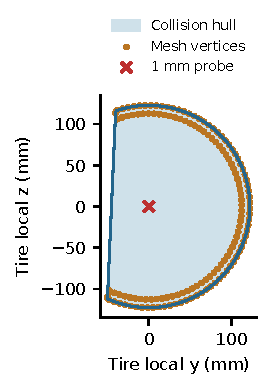
\includegraphics[width=\columnwidth]{collision.pdf}
\caption{Actual compiled tire vertices projected into the sector plane, and their convex hull. The single-mesh collision proxy fills the inner cavity. The missing circular cap remains, so this proxy is also distinct from a complete cylindrical wheel. The probe at the axle center detects a collision although this point is not tire material.}
\label{fig:collision}
\end{figure}

Flat support can still exercise the outer-sector geometry and finite angular range, because convexification preserves support in a plane-normal direction. However, the model cannot substantiate an inner-arc hooking mechanism. Most link and motor geoms also have collision disabled; only the upper/lower chassis and six tires are active robot collision geoms. Consequently, the tests do not establish whole-leg self-collision clearance. No hinge has a physical hard-stop constraint in the MJCF. Bounded commands do not replace those missing mechanical constraints.

\section{Travel Allocation and Finite-Sector Scheduling}
\subsection{One Contact-Travel Budget}
Let the filtered planar body command be $\vct{c}=[v_x,v_y,\omega_z]^\top$ and let $\vct{p}_i=[x_i,y_i]^\top$ denote a nominal contact relative to the footprint centroid. The required ground-contact travel relative to the body is
\begin{equation}
 \vct{u}_i=-\begin{bmatrix}v_x-\omega_z y_i\\v_y+\omega_z x_i\end{bmatrix}.\label{eq:travel}
\end{equation}
The negative sign distinguishes contact travel from body translation. For each leg, both distal rotation signs are considered. Steering is clipped to $\pm35^\circ$, and the candidate whose planar rolling direction $\hat{\vct{d}}_i$ best aligns with $\vct{u}_i$ is selected. Ties favor smaller steering magnitude. The alignment score is
\begin{equation}
 A_i=\max\left(0,\hat{\vct{d}}_i^\top\vct{u}_i/\|\vct{u}_i\|\right).
\end{equation}
A moving leg qualifies for rolling when $A_i\ge0.70$ and it belongs to the allowed leg set. If fewer than two legs qualify, every leg steps. For forward motion, the unrestricted rule selects $\{1,2,5,6\}$; the middle pair $\{3,4\}$ remains in stepping roles. This assignment is a consequence of this mounting geometry and steering limit, not a universal property of hexapods.

Let $\beta_i\in[0,1]$ be rolling authority after derating near an angular limit. Before saturation, the allocation is
\begin{align}
 \vct{u}^{\rm roll}_i&=\beta_i(\vct{u}_i^\top\hat{\vct{d}}_i)\hat{\vct{d}}_i,\\
 \vct{u}^{\rm art}_i&=\vct{u}_i-\vct{u}^{\rm roll}_i.\label{eq:split}
\end{align}
Stepping legs have $\beta_i=0$. For rolling legs, the scalar component is converted to a sector rate using $r_i$ and the selected sign. The rate is clipped to $540^\circ$/s and the integrated angle is clipped to the usable sector interval. Crucially, articulation uses the travel associated with the \emph{clipped commanded increment}, rather than the unclipped requested rate:
\begin{equation}
 \vct{u}^{\rm art}_i=\vct{u}_i-
 s_i r_i\frac{\theta_{i,k+1}-\theta_{i,k}}{\Delta t}\hat{\vct{d}}_i.\label{eq:clipped}
\end{equation}
Here $s_i\in\{-1,1\}$ accounts for motor direction. The equality budgets commanded kinematic travel; it is not feedback from measured motor rotation or contact slip. Tracking lag therefore remains a source of transport error.

The residual is integrated into a stance offset and clipped to an elliptical workspace with longitudinal/lateral caps of 90/70 mm. Numerical inverse kinematics supplies the articulated joint angles. The sector offset is then \emph{added} to the distal joint target, and final commands are bounded to $[0^\circ,360^\circ]$. A $40^\circ$ distal-branch guard triggers re-solving from the stance branch when the warm start selects a distant IK solution. The approximate contact invariance quantified above motivates this construction. It is not a global inverse-kinematics proof: saturation and posture changes can still cause tracking error or nonconvergence.

\subsection{Finite Arc and Contact Schedule}
The base scheduler uses alternating tripods $\mathcal T_A=\{1,4,5\}$ and $\mathcal T_B=\{2,3,6\}$ with phase offsets of one half-cycle. For frequency $f=2$ Hz and duty factor $D=0.60$,
\begin{equation}
 \phi_i=(ft+\delta_i)\bmod1,\qquad
 \text{swing window: }\phi_i\ge D.
\end{equation}
The two swing windows do not overlap. A stepping leg uses every allocated swing window. A rolling leg remains in stance until it has consumed at least half its reserved arc budget or the command becomes insufficiently aligned with its latched rolling direction. Once reindexing begins it continues through that swing window. Role and steering changes occur at lift-off, avoiding an instantaneous commanded steering change while loaded.

The usable arc is scanned geometrically in $2^\circ$ increments until the lowest support rises by more than 2 mm. Arc and actuator margins are 20 and $15^\circ$. Planned reserve accounts for stance travel, a factor of 1.8, a minimum reserve of $35^\circ$, and the distance that a quintic swing rewind can accommodate under the commanded rate cap. Authority decays smoothly over the last $12^\circ$ using $S(a)=10a^3-15a^4+6a^5$. Swing height reaches 25 mm; the lift amplitude scales with required travel speed relative to $0.05\,\mathrm{m/s}$.

This schedule leaves at least the opposite tripod \emph{commanded} in stance. It does not guarantee three loaded contacts, a positive support-polygon margin, or dynamic stability. A compliant body can unload a scheduled foot. Those are physical outcomes and must be assessed separately from the phase schedule.

\begin{figure*}[t]
\centering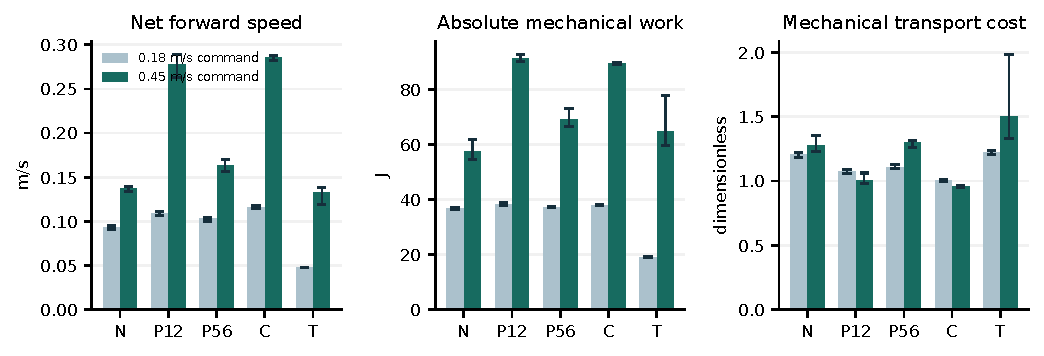
\includegraphics[width=0.96\textwidth]{results.pdf}
\caption{New deterministic phase-grid comparison on one unchanged model. Bars denote means over eight initial phases; whiskers span the observed minimum and maximum, not confidence intervals. All runs use the same 2 Hz cadence and 90/70 mm stride caps. The rolling-disabled condition shares the proposed scheduler; the separate tripod condition shares gait caps but uses a different scheduler and nominal foot construction.}
\label{fig:results}
\end{figure*}

\section{Experimental Method}
\subsection{Paired Development Grid}
The evaluation uses MuJoCo \MJVersion{}~\cite{todorov2012mujoco}, a 2 ms physics step, and a 20 ms target update. Each trial creates a fresh floating-base model, runs the initialization sequence, applies the common position-control setup, commands the nominal pose, and settles for 1 s with zero velocity command. The following 8 s include command-filter transients, role adoption, and locomotion. The command time constant is 0.15 s. The standard robot profile is used throughout.

Five conditions are compared: rolling disabled in the proposed scheduler (N), only IDs 1 and 2 allowed to roll (P12), only IDs 5 and 6 allowed to roll (P56), all geometrically qualified corner legs allowed (C), and a conventional tripod planner with the same frequency, duty factor, stride caps, command bounds, and shared motor setup (T). N/P12/P56/C differ only in the permitted rolling-leg set. Restricting that set changes steering, residual stroke, and swing skipping as part of the mechanism. Consequently, their differences test the combined allocation mechanism, not a pure distal-rotation effect with all joint trajectories held fixed. T is a secondary engineering control, not a fully matched causal ablation.

Both forward commands, $v_x\in\{0.18,0.45\}\,\mathrm{m/s}$, are crossed with phases $\phi_0=k/8$, $k=0,\ldots,7$, yielding 80 trials. All conditions share the same eight phases. The model parameters and terrain are nominal and deterministic; the phases are a fixed grid rather than samples from a population of robots or terrains. We therefore report means and full ranges, with paired differences, and do not attach population confidence intervals or infer success probabilities. There was no parameter retuning between these runs. This is a development evaluation of an existing candidate, not an independently held-out benchmark.

The run specification, dependency versions, source hashes, and Git dirty flag were recorded before execution. The source is not a clean release: the candidate controller is under development. A dedicated audit runner imports its class directly because the main package export and benchmark factory do not yet expose that path consistently. Results from that runner must not be described as successful execution of the separate locked ICRA benchmark. The raw records and source manifest are retained with the working manuscript; an anonymized, independently replayable release remains necessary before submission.

\subsection{Metrics and Interpretation}
The primary transport quantity is displacement along the initial chassis axis,
\begin{equation}
 \bar v_x^{\rm disp}=\frac{\vct{e}_x^\top R_0^\top[\vct{p}(T)-\vct{p}(0)]}{T}.
\end{equation}
It differs from peak velocity and from the mean velocity expressed in a continuously turning body frame. We independently integrate MuJoCo's world-frame body velocity and compare it to the position-derived value. Tracking RMSE uses per-step position differences transformed into the instantaneous body frame and compares against the original constant command; it includes the startup filter transient and gait-cycle velocity ripple.

Absolute mechanical work and its net-displacement normalization are
\begin{equation}
 W_{\rm abs}=\int_0^T\sum_{j=1}^{18}|\tau_j\dot q_j|dt,\qquad
 C_{\rm mt}=\frac{W_{\rm abs}}{mg\|\Delta\vct{p}_{xy}\|}.
\end{equation}
The normalization uses net planar displacement, so sideways drift can influence it. Absolute joint work counts both positive and negative work and is not measured battery energy or dissipated contact work.

Integrated slip averages the tangential speed over tire--ground contact points whose normal force exceeds 1 N and then integrates over time. This is a contact-point statistic, not a load-weighted energy integral or a per-wheel mean. Changing the number of contact points can affect the statistic. Uprightness is $u_z=\vct{e}_z^\top R\vct{e}_z$. A run terminates on nonfinite state or $u_z<\cos60^\circ$; completing this permissive test is not a deployment safety claim. We also record IK nonconvergence, stride clipping, lateral displacement, and yaw change rather than treating positive speed as sufficient success.

\begin{figure*}[t]
\centering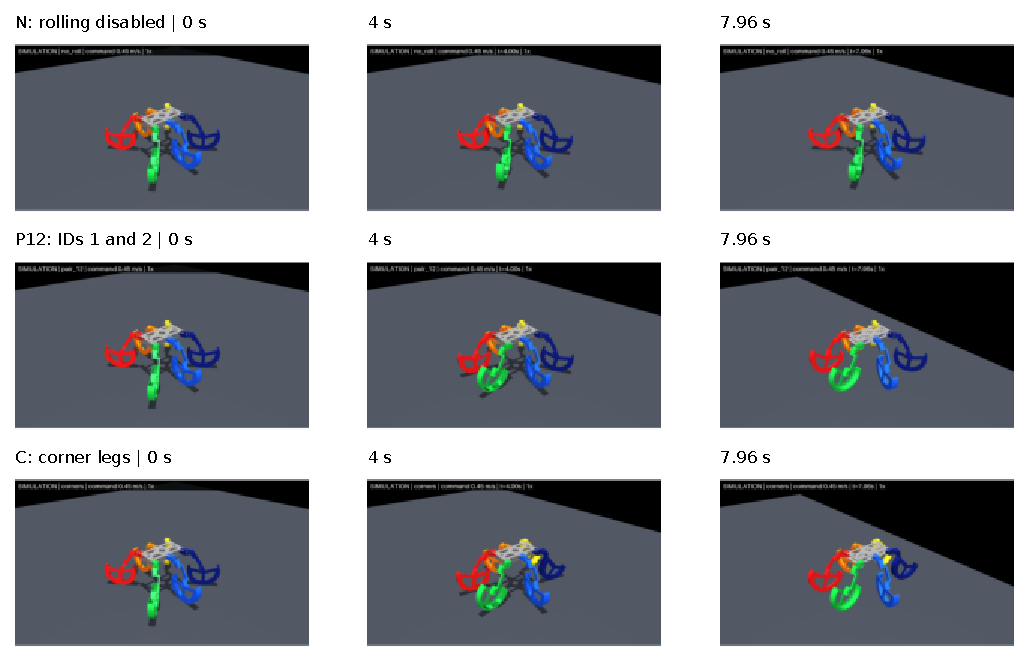
\includegraphics[width=0.98\textwidth]{replay.pdf}
\caption{Rendered replay of N, P12, and C under a 0.45 m/s command, at measurement times 0, 4, and 7.96 s. Each row is a separate trial at phase zero. A camera following the subtree center of mass keeps the robot visible; pixel displacement is not used to measure speed. Mesh colors identify model parts, not instantaneous support forces or selected rolling roles.}
\label{fig:replay}
\end{figure*}

\section{Results}
\subsection{Transport Across the Phase Grid}
Table~\ref{tab:speed} reports the same eight phases for every condition. At the high command, C reaches 0.285 m/s, 2.07 times N; P12 reaches 0.278 m/s, or 97.3\% of C. At the lower command, C reaches 0.116 m/s against 0.093 m/s for N. These are observed condition means, not a maximum attainable speed. The ordering between the two allowed pairs favors P12 for both tested commands; it need not persist at other commands or geometries.

\begin{table}[t]
\caption{Net forward speed: mean [min, max] over eight phases}
\label{tab:speed}\centering\small
\begin{tabular}{lcc}\toprule
Condition & $v_x^c=0.18$ m/s & $v_x^c=0.45$ m/s\\\midrule
N & 0.093 [0.091, 0.095] & 0.137 [0.134, 0.140]\\
P12 & 0.108 [0.107, 0.111] & 0.278 [0.263, 0.289]\\
P56 & 0.103 [0.100, 0.104] & 0.163 [0.157, 0.170]\\
C & 0.116 [0.114, 0.118] & 0.285 [0.283, 0.288]\\
T & 0.048 [0.047, 0.048] & 0.133 [0.119, 0.138]\\
\bottomrule\end{tabular}\end{table}

Pairing each phase with its N counterpart gives the high-command C-minus-N speed difference 0.148 m/s, spanning [0.144, 0.149] m/s over the grid. The analogous P12-minus-N difference is 0.140 m/s. These ranges describe sensitivity to the tested starting phases; they are not confidence intervals. The largest discrepancy between the velocity-integral diagnostic and displacement speed over all runs is 0.0023 m/s. All reported primary speeds are computed directly from net displacement.

\subsection{Tracking, Work, and Slip}
\begin{table}[t]
\caption{High-command metrics, means over eight phases}
\label{tab:cost}\centering\small
\begin{tabular}{lrrrr}\toprule
Condition & RMSE (m/s) & $W_{\rm abs}$ (J) & $C_{\rm mt}$ & Slip (m)\\\midrule
N & 0.318 & 57.331 & 1.277 & 0.383\\
P12 & 0.189 & 91.037 & 1.004 & 0.581\\
P56 & 0.299 & 69.160 & 1.299 & 0.528\\
C & 0.188 & 89.325 & 0.958 & 0.630\\
T & 0.324 & 64.752 & 1.500 & 0.456\\
\bottomrule\end{tabular}\end{table}

The faster configuration is not cheaper over the fixed eight-second window. C uses 89.3 J against 57.3 J for N, while transporting farther. Its mechanical cost of transport is 0.958 against 1.277, a different normalization with a different interpretation. Thus the result supports neither a blanket efficiency claim nor a claim that the speed gain is free. C also accumulates 0.630 m of contact-point slip against 0.383 m for N. The travel subtraction in the planner does not enforce a no-slip physical constraint.

The high-command tracking RMSE is 0.188 m/s for C and 0.318 m/s for N. Even when relative tracking improves, the commanded 0.45 m/s is not achieved. C's high-command yaw change ranges from -3.83 to 4.96 degrees; its largest lateral displacement is 0.147 m. Net forward transport, directional accuracy, and mechanical work must therefore be evaluated together.

\subsection{Execution and Scope}
All 80 trials complete their eight-second windows without nonfinite state or the 60-degree tilt termination. There are 0 recorded IK-nonconvergent control frames and 0 recorded forbidden chassis/ground collision steps. Minimum uprightness across the complete grid is 0.99921, and the minimum scheduled stance count is 3. These are finite-horizon model outcomes, not a population success rate or proof that scheduled feet always carry load.

A separate whole-project test run reports 259 passing test cases and one module-import error among 260 executed test entries. The latest candidate test module is not collected successfully through the public package. This packaging failure is distinct from the direct-run simulation data above, and remains a reproducibility issue to resolve before an external release.


\subsection{Numerical Sensitivity and Visual Replay}
After the main grid, we repeated N, P12, and C at phase zero using 1, 2, and 4 ms physics steps with the same 20 ms target update, initialization, and 8 s measurement. These nine supplementary development trials completed. Across those steps the observed speed ranges were 0.1351--0.1361, 0.2883--0.2891, and 0.2825--0.2831 m/s, respectively. The largest change from the 2 ms value was below 0.00085 m/s. This bounds timestep sensitivity for three nominal trials; it is not a convergence proof for other contacts or terrains. At this particular phase P12 exceeds C slightly, whereas C is faster in the eight-phase mean; the replay is not a replacement for the complete grid.

Figure~\ref{fig:replay} shows actual renderings of the same phase-zero trials. Their position-derived speeds exactly reproduce the original records to the checked numerical tolerance ($10^{-9}$ m/s). The accompanying video labels simulation and archival hardware separately, retains normal playback speed, and reports the command independently from achieved speed.



\begin{figure*}[t]
\centering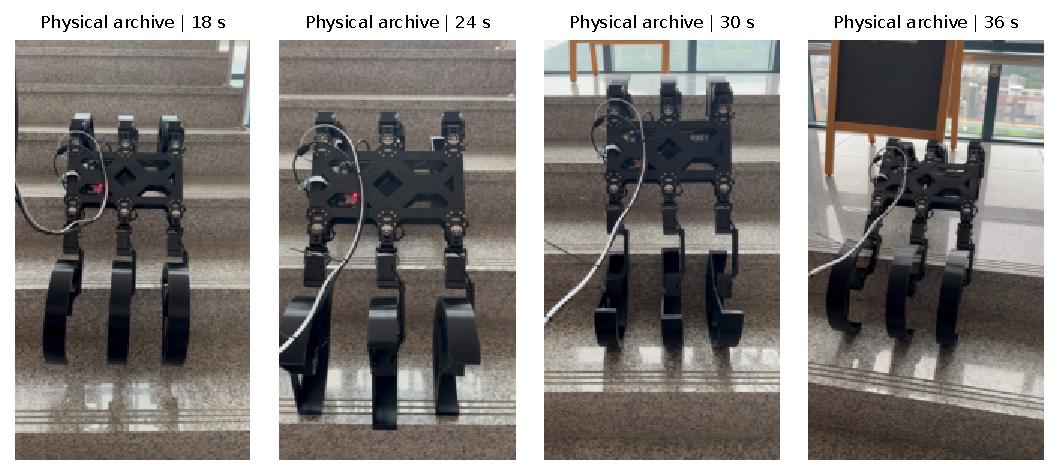
\includegraphics[width=0.98\textwidth]{hardware_stairs.pdf}
\caption{Archival physical stair-motion sequence, at source-video times 18, 24, 30, and 36 s. Frames are presented in their original order and without geometric retouching. This is qualitative prototype evidence under an undocumented historical controller, not part of the 80 simulation trials or a controlled comparison with a closed wheel. The visible cable and moving camera are retained.}
\label{fig:stairs}
\end{figure*}

\section{Discussion and Limitations}
\subsection{What the Comparison Establishes}
The role-subset experiment addresses whether the shared distal joint can supply useful transport while the remaining articulation accommodates the residual contact motion. Within this controller and model, the most informative control is rolling disabled in the same scheduler. A favorable comparison to the slower secondary tripod condition alone would not establish the mechanism, because the schedulers and nominal support constructions differ. Nor should the high-speed command be interpreted as a claimed attainable tracking target: achieved motion remains substantially below $0.45\,\mathrm{m/s}$.

The two-leg condition is useful for actuator allocation, but all eighteen actuators remain installed and the nominally nonrolling distal joints still articulate during stepping. It therefore demonstrates fewer legs assigned to rolling, not a twelve- or sixteen-actuator physical robot, and not a measured power saving from removing hardware. The paired subsets are identified by model IDs; changing the body-frame convention can reverse informal front/rear labels.

\subsection{Stairs and Morphological Attribution}
Figure~\ref{fig:stairs} presents four frames from an archival physical stair sequence. It shows a real open-arc prototype in changing stair-contact configurations, with an external cable visible throughout. The camera moves with the robot, and the recording provides no synchronized control log or verified stair calibration. It cannot establish the new controller's success rate, achieved stair height, autonomy, energy use, or a causal benefit from the inner opening.



Earlier development simulations in this project recorded stair top-reaching under a different controller revision. They are not pooled with the new role-allocation results. In particular, a riser taller than the outer radius does not establish an advantage from an opening. For an idealized circular wheel pivoting at an accessible sharp edge,
\begin{equation}
 \tau_a+F_h(r-h)\ge F_i\sqrt{2rh-h^2}
\end{equation}
is a necessary quasi-static moment condition. Here $r$ is wheel radius, $h$ is edge height, $F_i$ is downward axle load, $F_h$ is a forward horizontal axle force, and $\tau_a$ is the driving torque. The expression assumes $0<h<2r$ and an accessible edge pivot. The force-only expression becomes singular near $h=r$ when $\tau_a=0$; allowing axle torque changes that conclusion. Edge accessibility, friction, articulation, and contact geometry still constrain ascent. The chord length $2r\sin(\psi/2)$ for a subtended angle $\psi$ is a geometric descriptor, not a general criterion for hooking or a maximum riser height. A plane-preserving convex hull cannot resolve concave edge capture. A decomposed tire and a matched closed-wheel control with verified contact events are necessary for that research question.

\subsection{External Validity and Remaining Validation}
The study varies initial phase on flat ground only. It does not establish robustness to mass, friction, actuator strength, changing commands, slopes, or uneven terrain. The nominal friction and contact softness are not identified from the assembled robot. The model omits many self-collisions and hard stops, and stall-matched actuator saturation does not reproduce thermal limits, gearbox losses, battery sag, or structural compliance. The additional timestep check covers only phase-zero flat-ground trials; a different contact representation could still change the outcomes. The current results therefore motivate, but cannot replace, hardware comparisons and broader numerical convergence studies.

A stronger follow-up would freeze one executable release, identify the mechanically permitted ranges, compare at several target speeds under calibrated perturbations, and separately ablate role selection, travel subtraction, and reindexing. Actual loaded support, sector-edge contact events, joint tracking, and electrical energy should be measured. A dedicated continuous-wheel baseline should preserve actuator and inertial budgets, while being allowed its own valid contact model. Contact-shape comparisons need controller-independent geometry handling; simply replacing a mesh with a cylinder can violate this controller's mesh-based calibration assumptions.

\section{Conclusion}
We presented a finite-sector controller that assigns rolling and stepping roles and divides each contact's required travel between distal rotation and articulation. A matched-phase simulation study quantifies the resulting transport, tracking, work, and slip trade-offs. The contribution is a bounded control mechanism on one development model. Its convex collision proxy cannot substantiate inner-arc hooking; controlled hardware comparisons and morphology-specific validation remain open.

\noindent\begin{minipage}{\columnwidth}
\section*{Acknowledgment of AI Assistance}
OpenAI Codex was used to draft and revise the Abstract and Sections I--VIII, organize source-based analysis, and generate audit, plotting, and video-composition code for this working manuscript. The figures combine deterministic diagrams, data plots, direct simulation renders, and archival project media; no physical robot image or experimental observation was synthesized by an image generator. Numerical values were obtained by executing simulation or geometry calculations, not synthesized as experimental observations. The authors must verify the manuscript, references, code, and figures before submission and retain responsibility for the final work.

\end{minipage}

\IEEEtriggeratref{7}
\bibliographystyle{IEEEtran}
\bibliography{references}
\end{document}
